\section{Results and Analysis}
We validated our system's conversion using scenes from Bitterli's 32 resources 
\cite{resources16}. We chose scenes that provided a wide variety of directives 
in order to cover most commonly used directives. These scenes include: different 
types of materials and bumpmaps; 3D meshes and primitive shapes; image and 
primitive textures; area and environment lighting. 

The scenes were rendered using Mitsuba 0.5.0, PBRT v3 and LuxRender v1.6 on 
%a UNIX system running
Ubuntu 14.04 LTS. All scenes were rendered using over 5,000 samples per pixel. 

\begin{figure*}
\centering
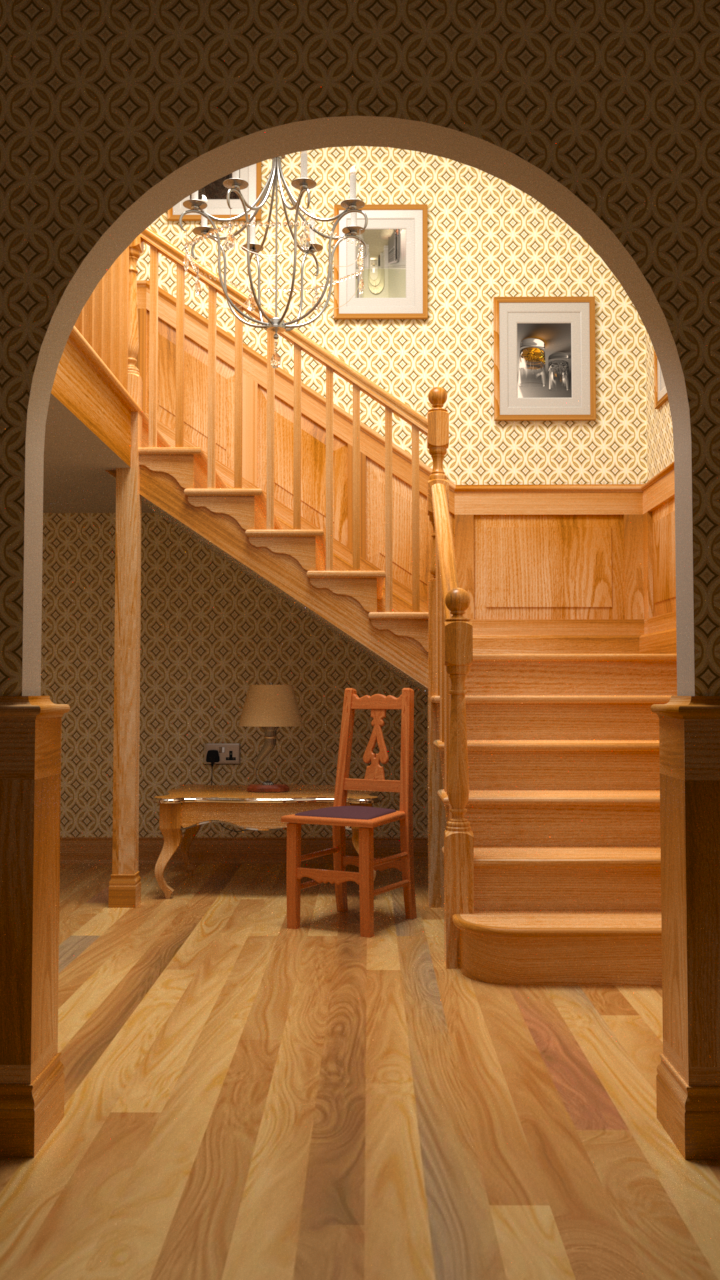
\includegraphics[width=1.5in]{figs/4_results/staircase/1_from_lux.png}
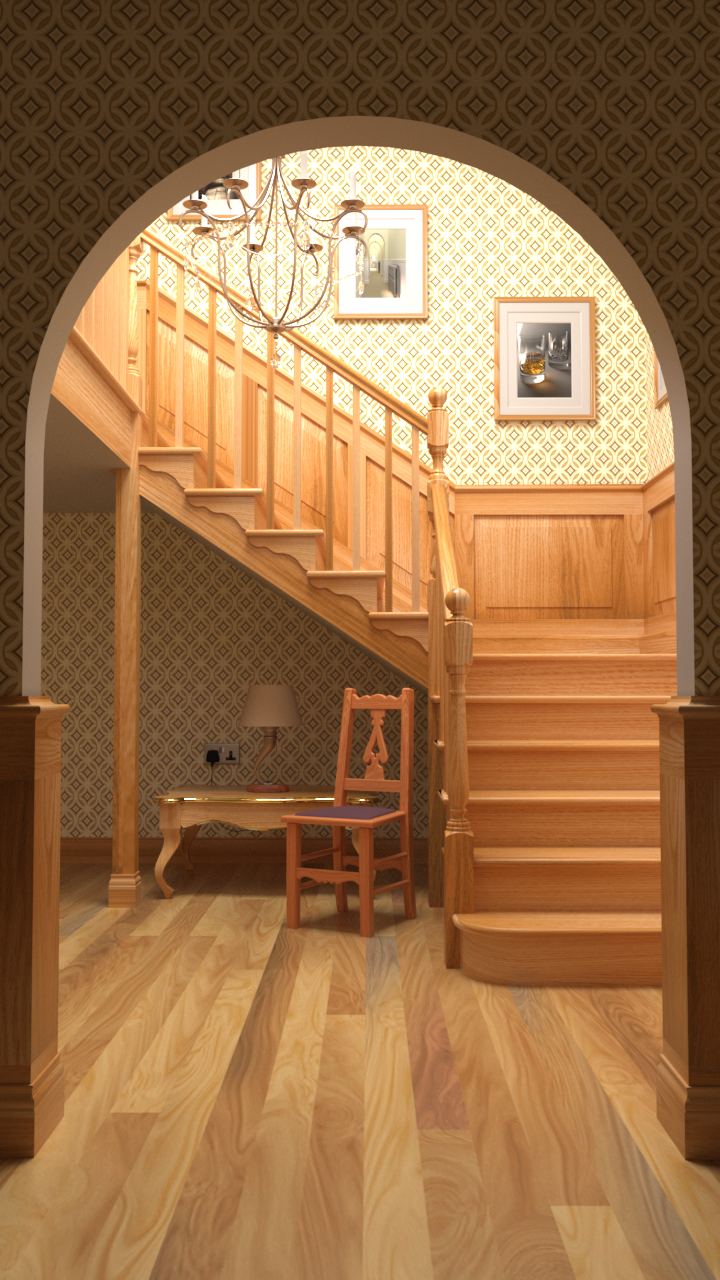
\includegraphics[width=1.5in]{figs/4_results/staircase/2_to_mitsuba.png}
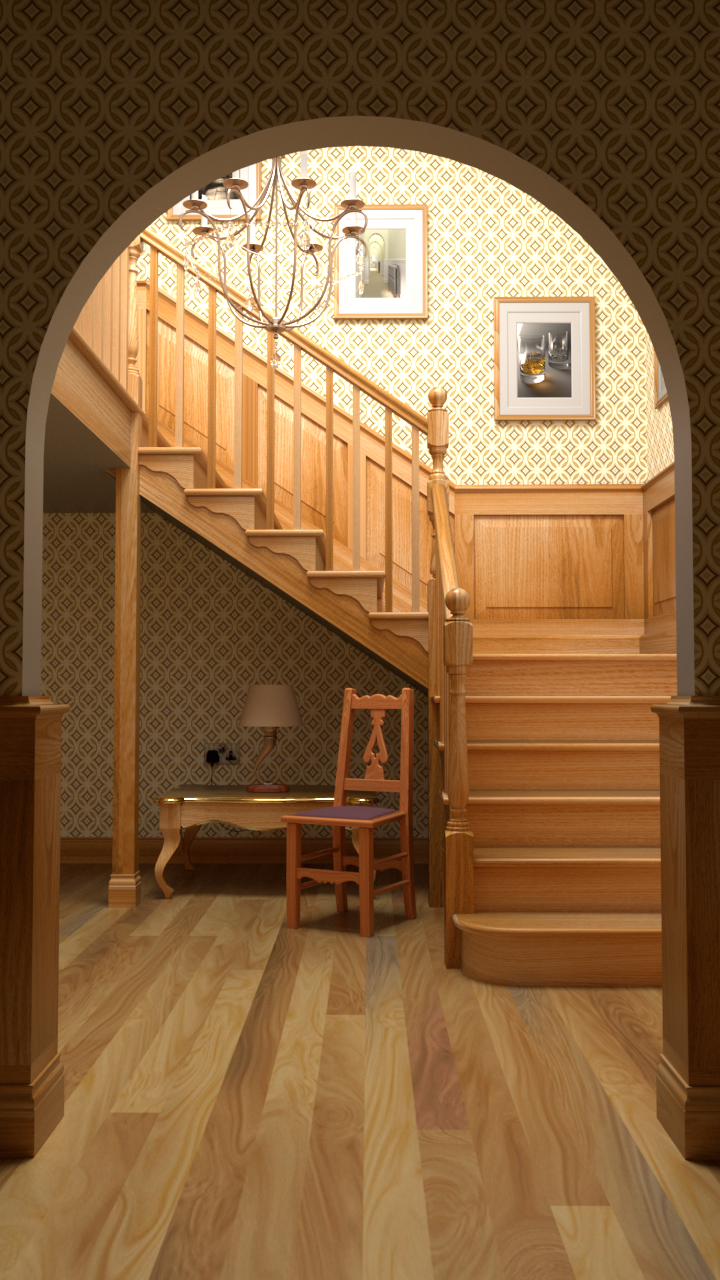
\includegraphics[width=1.5in]{figs/4_results/staircase/3_to_pbrt.png}
\caption{Automatic conversion obtained with our system for \textit{The Wooden Staircase}
scene, originally modeled for LuxRender. Rendering produced by LuxRender (left).
Rendering produced by Mitsuba (center) and PBRT v3 (right),
from converted scenes for the renderers}
\label{fig:staircase}
\end{figure*}

\begin{figure*}
\centering
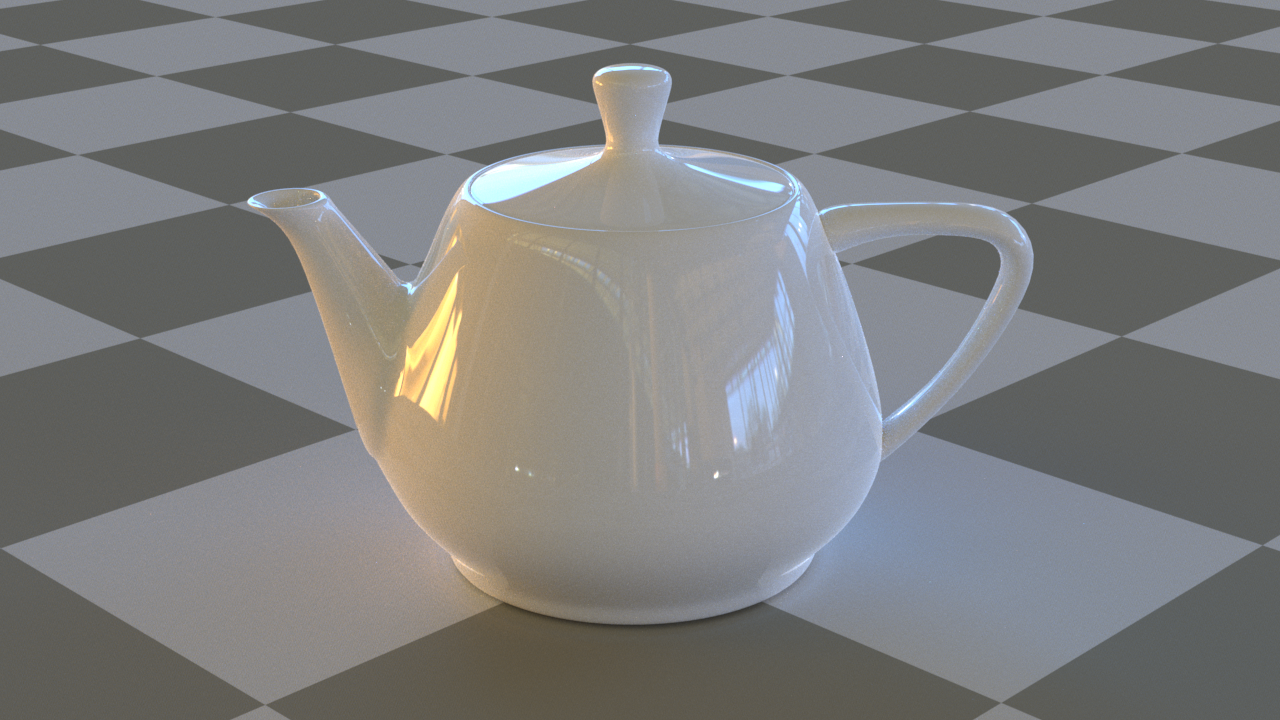
\includegraphics[width=2in]{figs/4_results/teapot/1_from_lux.png}
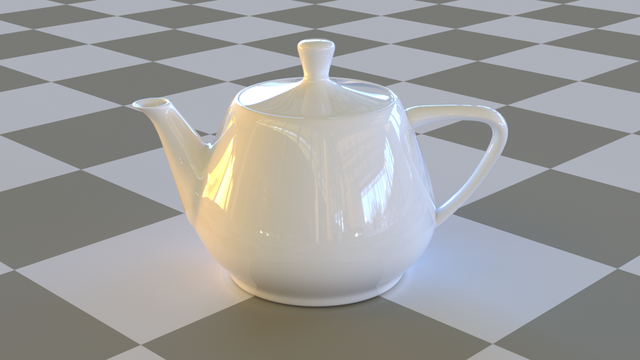
\includegraphics[width=2in]{figs/4_results/teapot/2_to_mitsuba.png}
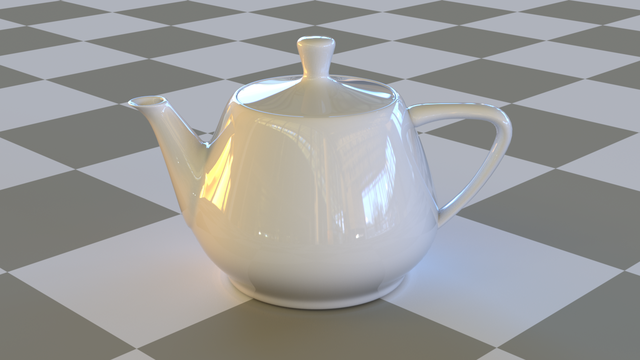
\includegraphics[width=2in]{figs/4_results/teapot/3_to_pbrt.png}
\caption{Automatic conversion obtained with our system for \textit{Utah Teapot}
scene originally modeled for LuxRender. Rendering produced by LuxRender (left).
Rendering produced by Mitsuba (center) and PBRT v3 (right),
from converted scenes for the renderers}
\label{fig:teapot}
\end{figure*}

\begin{figure*}
\centering
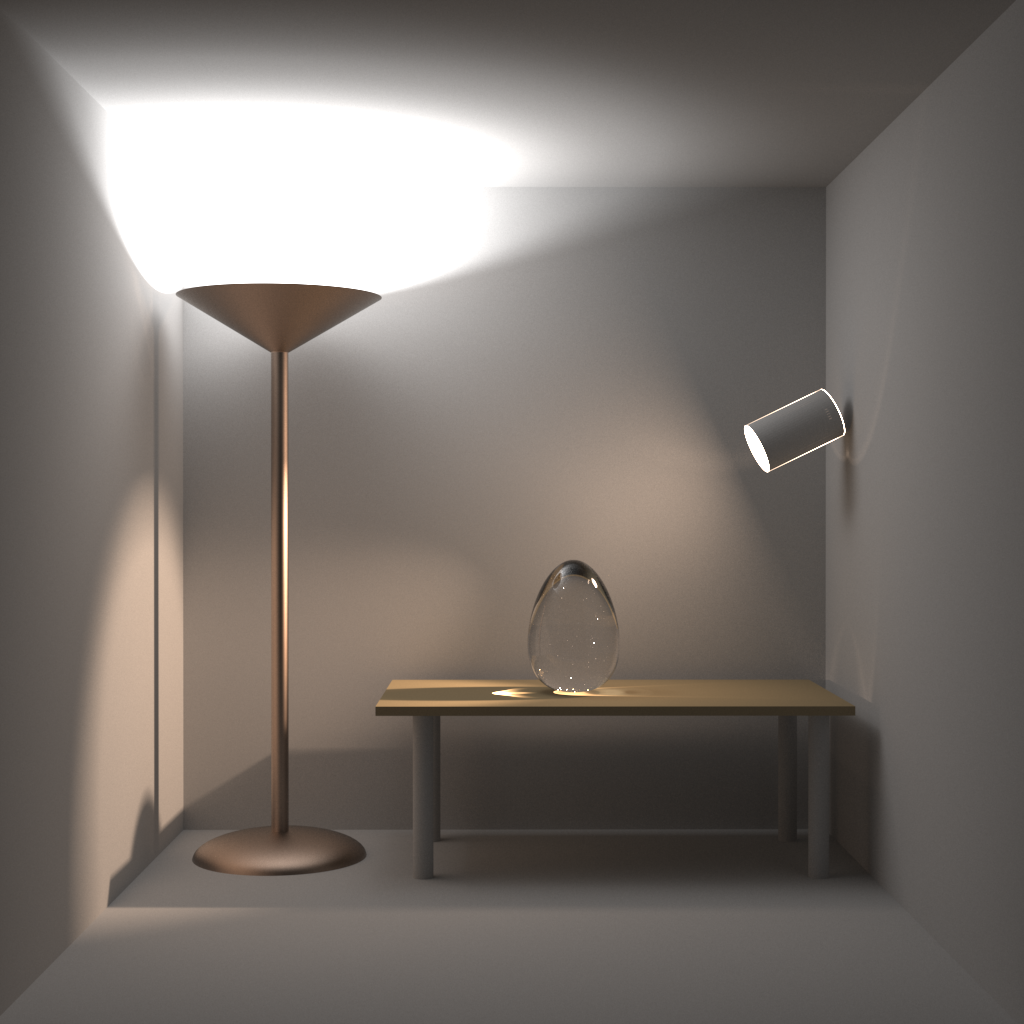
\includegraphics[width=2in]{figs/4_results/veach-bidir/1_from_mitsuba.png}
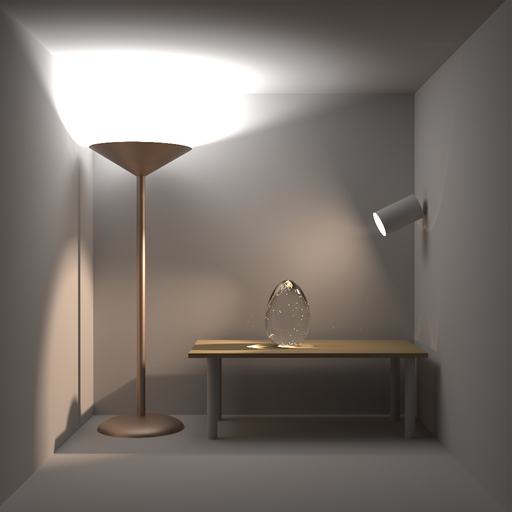
\includegraphics[width=2in]{figs/4_results/veach-bidir/2_to_pbrt.png}
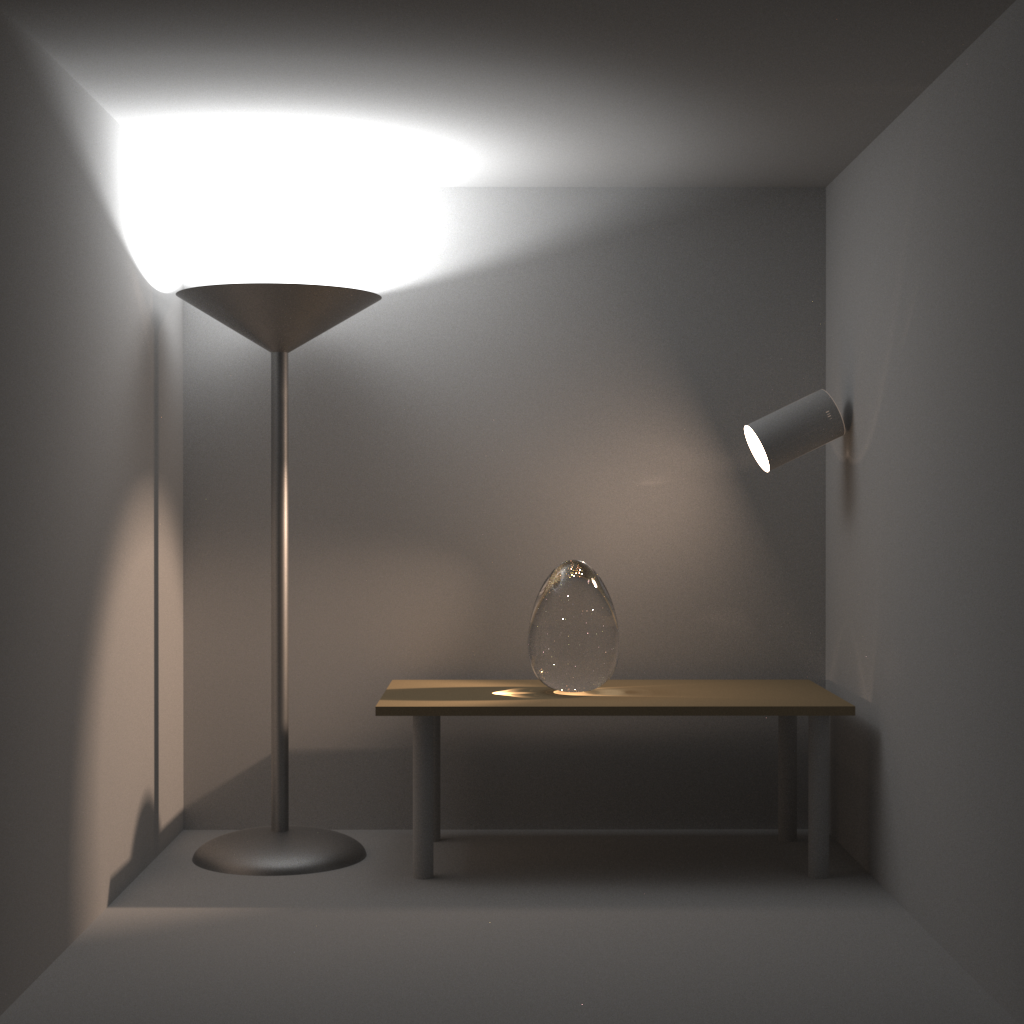
\includegraphics[width=2in]{figs/4_results/veach-bidir/3_to_lux.png}
\caption{Automatic conversion obtained with our system for \textit{Veach, Bidir Room}
scene originally modeled for Mitsuba. Rendering produced by Mitsuba (left).
Rendering produced by PBRT v3 (center) and LuxRender (right),
from converted scenes for the renderers}
\label{fig:veach-bidir}
\end{figure*}

%\begin{figure*}
%\centering
%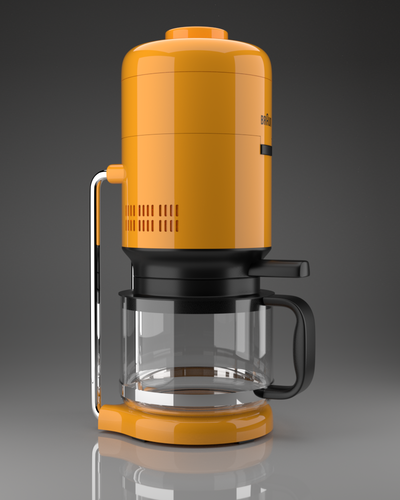
\includegraphics[width=2in]{figs/4_results/coffee/1_from_pbrt.png}
%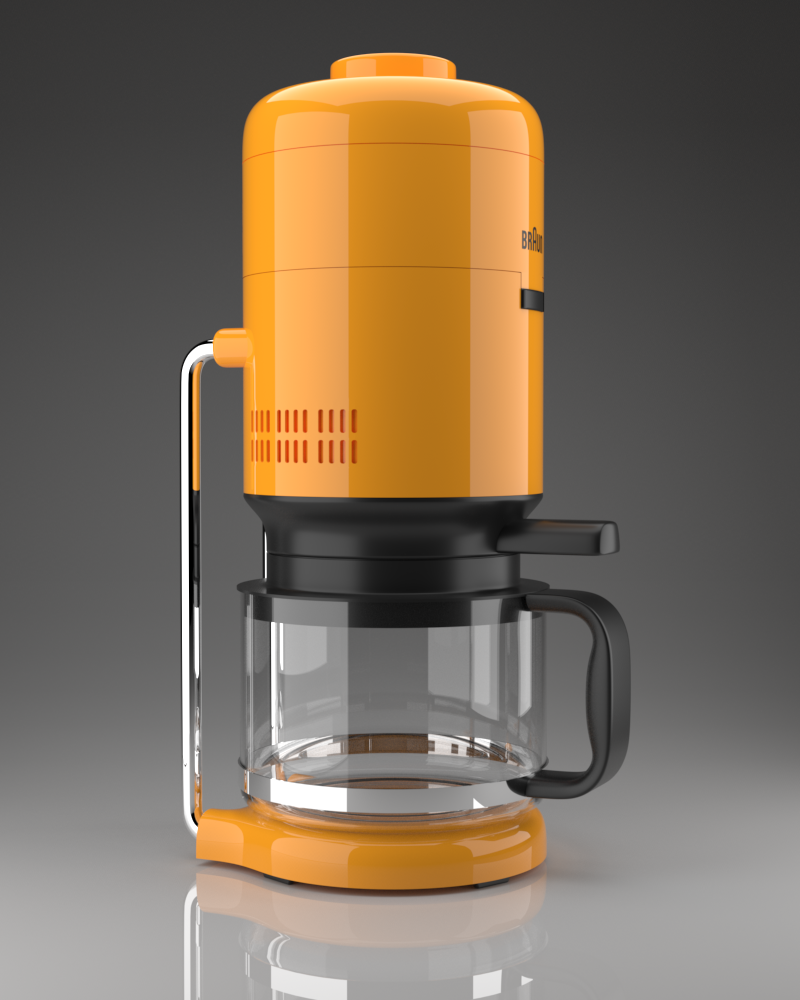
\includegraphics[width=2in]{figs/4_results/coffee/2_to_mitsuba.png}
%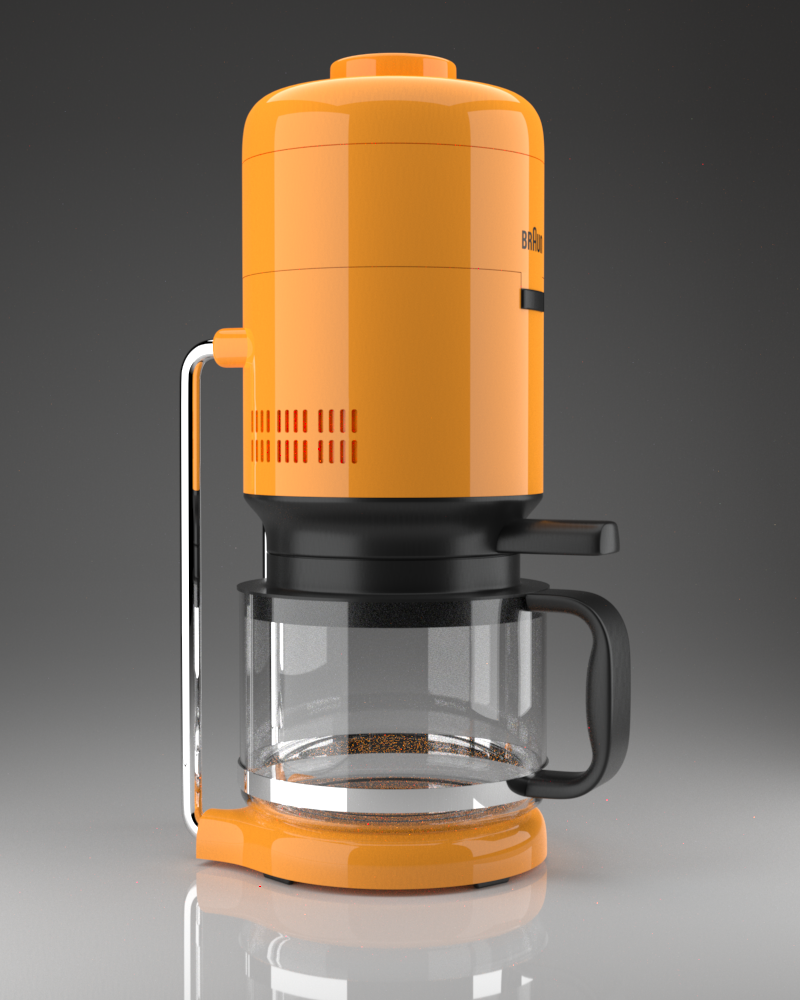
\includegraphics[width=2in]{figs/4_results/coffee/3_to_lux.png}
%\caption{Automatic conversion obtained with our system for \textit{Coffee Maker}
%scene originally modeled for PBRT v3. Rendering produced by PBRT v3 (left).
%Rendering produced by Mitsuba (center) and LuxRender (right),
%from converted scenes for the renderers}
%\label{fig:coffee}
%\end{figure*}

\begin{figure*}
\centering
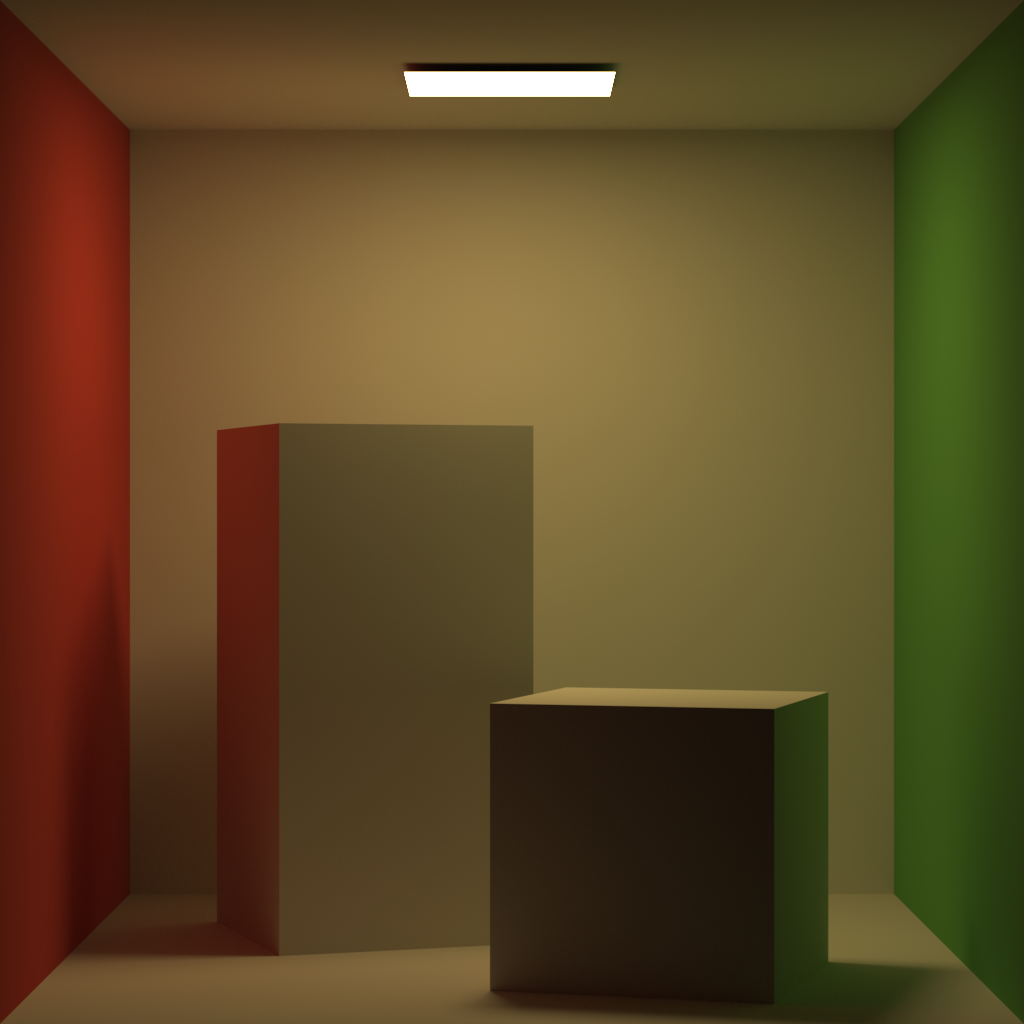
\includegraphics[width=2in]{figs/4_results/cornell-box/1_from_mitsuba.png}
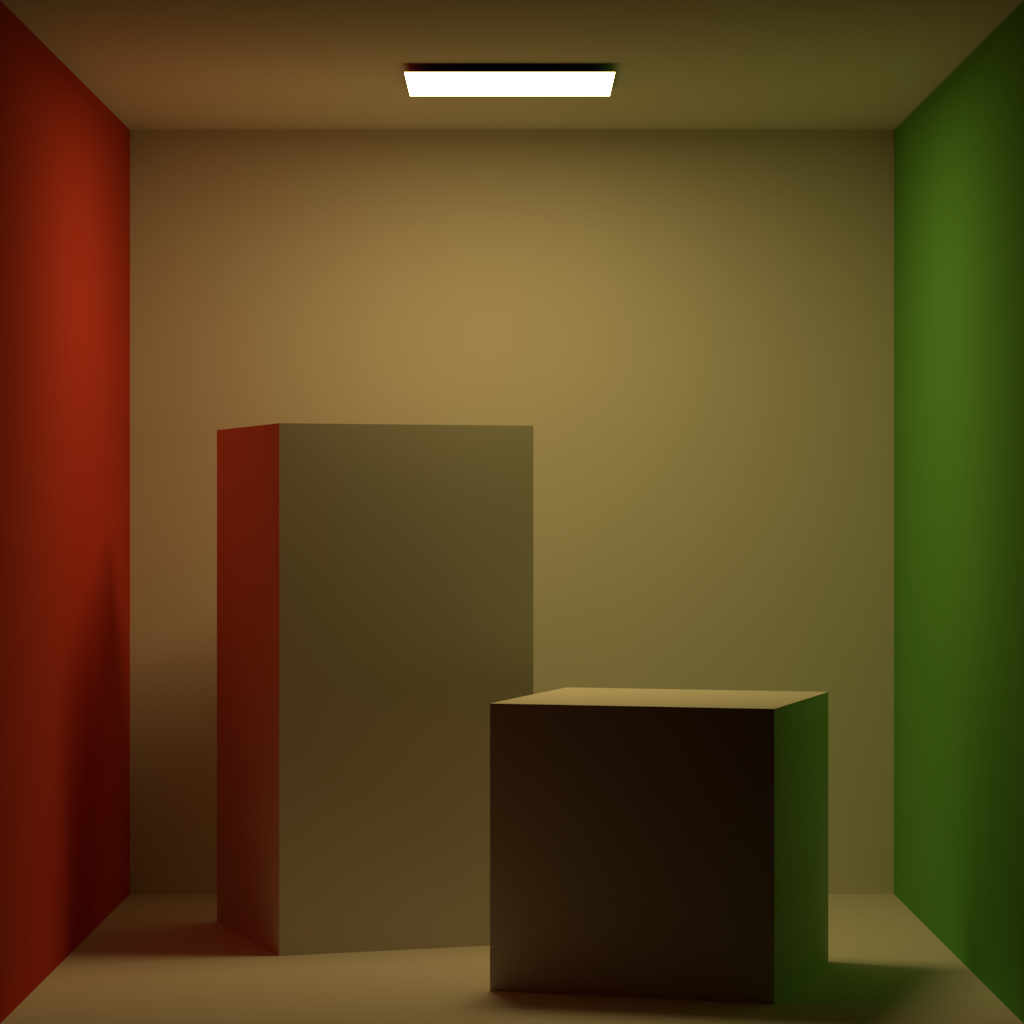
\includegraphics[width=2in]{figs/4_results/cornell-box/2_to_pbrt.png}
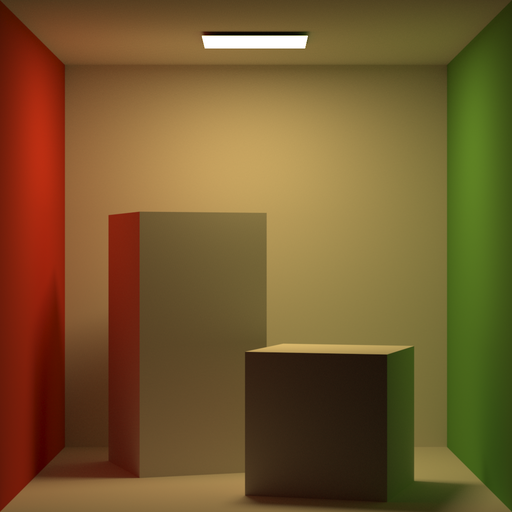
\includegraphics[width=2in]{figs/4_results/cornell-box/3_to_lux.png}
\caption{Automatic conversion obtained with our system for \textit{Cornell Box}
scene originally modeled for Mitsuba. Rendering produced by Mitsuba (left).
Rendering produced by PBRT v3 (center) and LuxRender (right),
from converted scenes for the renderers}
\label{fig:coffee}
\end{figure*}

\subsection{Limitations}
In order to minimize scope issues, we restricted the number of directives 
interpreted by our system. Generally speaking, directives present in only one 
renderer that had no correspondent in the other two renderers were not 
incorporated. That was the case, for instance, for Mitsuba-only materials like 
\textit{phong} or \textit{blendbsdf}. 

We chose not to interpret and convert hair or participating media (volumes, such 
as water or fog) for this PoC. We also did not convert the color for metal 
materials in LuxRender given the issues discussed in \ref{systemarch}. The 
latter can be observed in Figure \ref{fig:coffee} - we can see the lack of a 
copper color on the lamp in the image rendered by LuxRender.




